\documentclass[journal, a4paper]{IEEEtran}

% some very useful LaTeX packages include:

%\usepackage{cite}      % Written by Donald Arseneau
                        % V1.6 and later of IEEEtran pre-defines the format
                        % of the cite.sty package \cite{} output to follow
                        % that of IEEE. Loading the cite package will
                        % result in citation numbers being automatically
                        % sorted and properly "ranged". i.e.,
                        % [1], [9], [2], [7], [5], [6]
                        % (without using cite.sty)
                        % will become:
                        % [1], [2], [5]--[7], [9] (using cite.sty)
                        % cite.sty's \cite will automatically add leading
                        % space, if needed. Use cite.sty's noadjust option
                        % (cite.sty V3.8 and later) if you want to turn this
                        % off. cite.sty is already installed on most LaTeX
                        % systems. The latest version can be obtained at:
                        % http://www.ctan.org/tex-archive/macros/latex/contrib/supported/cite/

\usepackage{graphicx}   % Written by David Carlisle and Sebastian Rahtz
                        % Required if you want graphics, photos, etc.
                        % graphicx.sty is already installed on most LaTeX
                        % systems. The latest version and documentation can
                        % be obtained at:
                        % http://www.ctan.org/tex-archive/macros/latex/required/graphics/
                        % Another good source of documentation is "Using
                        % Imported Graphics in LaTeX2e" by Keith Reckdahl
                        % which can be found as esplatex.ps and epslatex.pdf
                        % at: http://www.ctan.org/tex-archive/info/

%\usepackage{psfrag}    % Written by Craig Barratt, Michael C. Grant,
                        % and David Carlisle
                        % This package allows you to substitute LaTeX
                        % commands for text in imported EPS graphic files.
                        % In this way, LaTeX symbols can be placed into
                        % graphics that have been generated by other
                        % applications. You must use latex->dvips->ps2pdf
                        % workflow (not direct pdf output from pdflatex) if
                        % you wish to use this capability because it works
                        % via some PostScript tricks. Alternatively, the
                        % graphics could be processed as separate files via
                        % psfrag and dvips, then converted to PDF for
                        % inclusion in the main file which uses pdflatex.
                        % Docs are in "The PSfrag System" by Michael C. Grant
                        % and David Carlisle. There is also some information
                        % about using psfrag in "Using Imported Graphics in
                        % LaTeX2e" by Keith Reckdahl which documents the
                        % graphicx package (see above). The psfrag package
                        % and documentation can be obtained at:
                        % http://www.ctan.org/tex-archive/macros/latex/contrib/supported/psfrag/

%\usepackage{subfigure} % Written by Steven Douglas Cochran
                        % This package makes it easy to put subfigures
                        % in your figures. i.e., "figure 1a and 1b"
                        % Docs are in "Using Imported Graphics in LaTeX2e"
                        % by Keith Reckdahl which also documents the graphicx
                        % package (see above). subfigure.sty is already
                        % installed on most LaTeX systems. The latest version
                        % and documentation can be obtained at:
                        % http://www.ctan.org/tex-archive/macros/latex/contrib/supported/subfigure/

\usepackage{url}        % Written by Donald Arseneau
                        % Provides better support for handling and breaking
                        % URLs. url.sty is already installed on most LaTeX
                        % systems. The latest version can be obtained at:
                        % http://www.ctan.org/tex-archive/macros/latex/contrib/other/misc/
                        % Read the url.sty source comments for usage information.

%\usepackage{stfloats}  % Written by Sigitas Tolusis
                        % Gives LaTeX2e the ability to do double column
                        % floats at the bottom of the page as well as the top.
                        % (e.g., "\begin{figure*}[!b]" is not normally
                        % possible in LaTeX2e). This is an invasive package
                        % which rewrites many portions of the LaTeX2e output
                        % routines. It may not work with other packages that
                        % modify the LaTeX2e output routine and/or with other
                        % versions of LaTeX. The latest version and
                        % documentation can be obtained at:
                        % http://www.ctan.org/tex-archive/macros/latex/contrib/supported/sttools/
                        % Documentation is contained in the stfloats.sty
                        % comments as well as in the presfull.pdf file.
                        % Do not use the stfloats baselinefloat ability as
                        % IEEE does not allow \baselineskip to stretch.
                        % Authors submitting work to the IEEE should note
                        % that IEEE rarely uses double column equations and
                        % that authors should try to avoid such use.
                        % Do not be tempted to use the cuted.sty or
                        % midfloat.sty package (by the same author) as IEEE
                        % does not format its papers in such ways.

\usepackage{amsmath}    % From the American Mathematical Society
                        % A popular package that provides many helpful commands
                        % for dealing with mathematics. Note that the AMSmath
                        % package sets \interdisplaylinepenalty to 10000 thus
                        % preventing page breaks from occurring within multiline
                        % equations. Use:
%\interdisplaylinepenalty=2500
                        % after loading amsmath to restore such page breaks
                        % as IEEEtran.cls normally does. amsmath.sty is already
                        % installed on most LaTeX systems. The latest version
                        % and documentation can be obtained at:
                        % http://www.ctan.org/tex-archive/macros/latex/required/amslatex/math/



% Other popular packages for formatting tables and equations include:

%\usepackage{array}
% Frank Mittelbach's and David Carlisle's array.sty which improves the
% LaTeX2e array and tabular environments to provide better appearances and
% additional user controls. array.sty is already installed on most systems.
% The latest version and documentation can be obtained at:
% http://www.ctan.org/tex-archive/macros/latex/required/tools/

% V1.6 of IEEEtran contains the IEEEeqnarray family of commands that can
% be used to generate multiline equations as well as matrices, tables, etc.

% Also of notable interest:
% Scott Pakin's eqparbox package for creating (automatically sized) equal
% width boxes. Available:
% http://www.ctan.org/tex-archive/macros/latex/contrib/supported/eqparbox/

% *** Do not adjust lengths that control margins, column widths, etc. ***
% *** Do not use packages that alter fonts (such as pslatex).         ***
% There should be no need to do such things with IEEEtran.cls V1.6 and later.


% Your document starts here!
\begin{document}

% Define document title and author
	\title{Kindle vs. iBooks: A Comparison in iOS Interaction Design}
	\author{Joshua Kuroda
	\thanks{Professor: ~John David N. Dionisio, PhD., Loyola Marymount University | Seaver College of Science \& Engineering - Computer Science}}
	\markboth{CMSI 370-01 Interaction Design - Assignment 0924}{}
	\maketitle

% Write abstract here
\begin{abstract}
	Two mobile e-book applications were analyzed side-by-side using a pool of 13 test subjects to measure learnability, satisfaction, and errors. These metrics would then allow one to conclude which application complied better with its respective guidelines documentation. In addition, the results would also point to an application that was better received by our users, on the basis of satisfactory (or unsatisfactory) comments.
\end{abstract}

% Each section begins with a \section{title} command
\section{Introduction}
	% \PARstart{}{} creates a tall first letter for this first paragraph
	\PARstart{T}{he} decision to use both the iBooks and Kindle applications on a mobile OS was made because of the ubiquity of mobile devices in the college environment and because of the fact that using both applications on their native devices would bring in more variables than necessary. Both applications are available on the Apple App Store for free and require iOS 7.0 or later. The results for this report reflect each application's performance on the iPhone 6, though both applications are available on the iPad and iPod touch. Although both applications may offer differing services and products, this report focuses on the main purpose of both: to offer an excellent reading experience on an electronic platform.

% Main Part
\section{Structure of Data}
	% LaTeX takes complete care of your document layout ...
	The metrics gathered are based off of three basic tasks that were asked of users when using either application: \\
    
    (1) Download a book, \\
    
    (2) Highlight and make a note in the text, and \\
    
    (3) Find a quote from the book. \\
    
    The book chosen for testing was \emph{Thrill}, by Lucia Jordan. This book is free and obscure enough to make sure that no users would be too familiar with the text. For each task, the time taken as well as the number of errors were recorded. Comments were also written down if applicable. 
	% ... but you can insert a line break manually with two backslashes, if needed: \\

\section{Results}
	% You can cite a book or paper by using \cite{reference}.
	% The references will be defined at the end of this .tex file in the bibliography
	%References should be cited as numbers, and should be ordered by their appearance (example: ``... as shown in \cite{HOP96}, ...'').
    Based on the following results, iBooks has been found to be the preferable reading application because of its overall performance compared to that of Kindle. In addition to the time taken for each task, other observations were prioritized as well. For the first task, accuracy and ease of the search feature were analyzed. The second task looked at the implementation of text selection menus. The third and final task prioritized quickness and precision, since most users want search features to have both of those qualities. The average metrics for all three tasks can be found in table~\ref{fig:averagesTable} and figure~\ref{fig:averagesGraph}.
    
    \begin{figure}[!hbt]
		% Center the figure.
		\begin{center}
		% Include the eps file, scale it such that it's width equals the column width. You can also put width=8cm for example...
		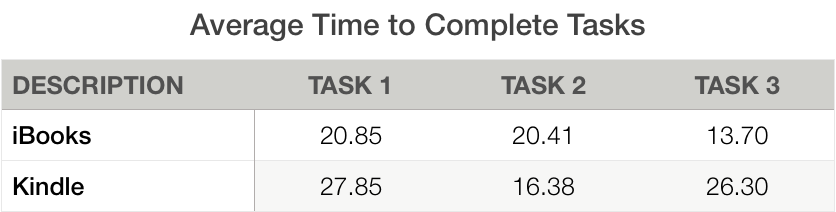
\includegraphics[width=8cm]{averagesTable}
		% Create a subtitle for the figure.
		\caption{Note: the above averages omit disturbing outliers.}
		% Define the label of the figure. It's good to use 'fig:title', so you know that the label belongs to a figure.
		\label{fig:averagesTable}
		\end{center}
	\end{figure}
    
    \begin{figure}[!hbt]
		% Center the figure.
		\begin{center}
		% Include the eps file, scale it such that it's width equals the column width. You can also put width=8cm for example...
		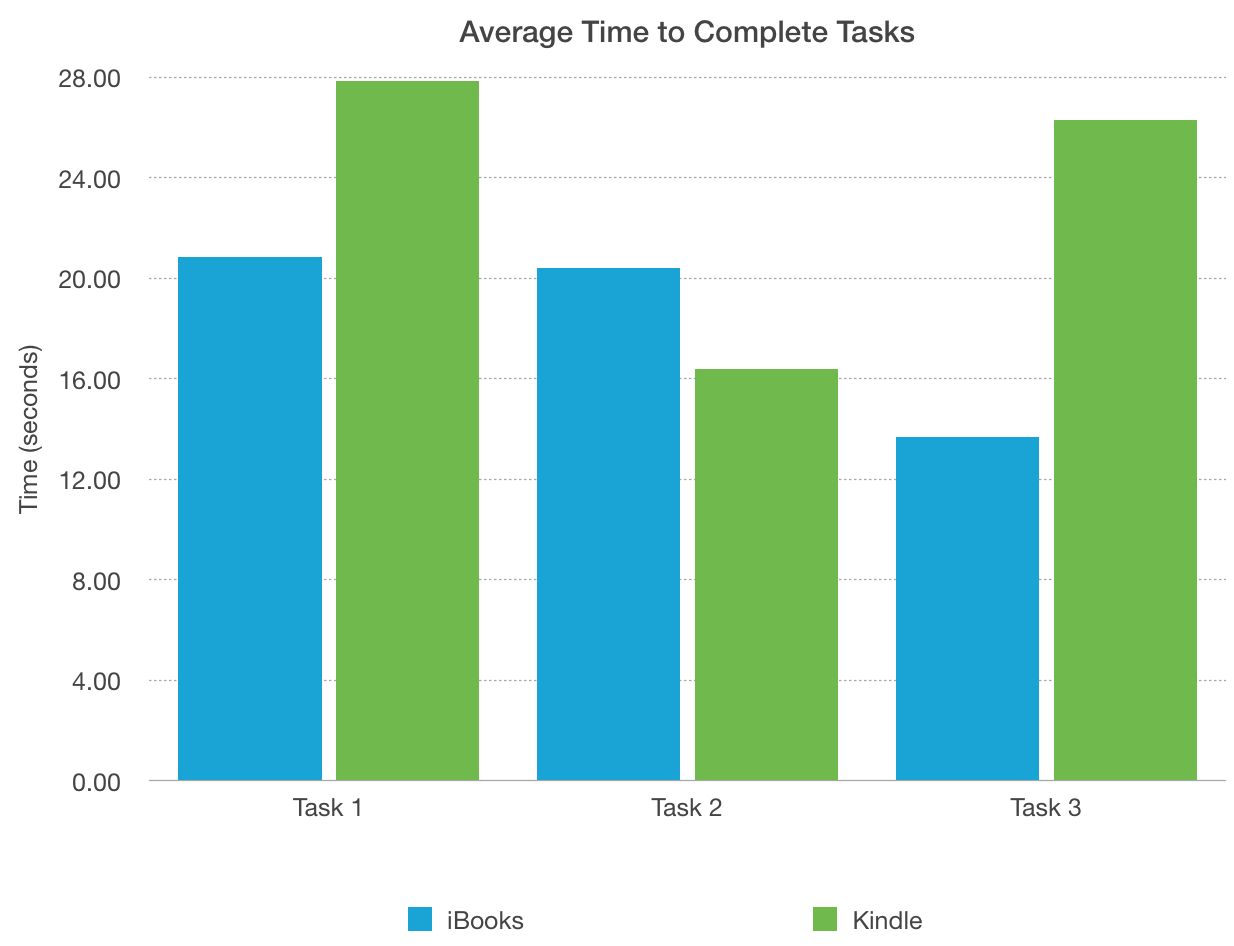
\includegraphics[width=8cm]{averagesGraph}
		% Create a subtitle for the figure.
		\caption{The compiled and averaged data collected from 13 test subjects.}
		% Define the label of the figure. It's good to use 'fig:title', so you know that the label belongs to a figure.
		\label{fig:averagesGraph}
		\end{center}
	\end{figure}
	
\subsection{Task 1: Download Book}
	Most users were new to both applications, so the learnability metric applied to the following data. First up was the task to download a book, which varied slightly between the applications. For iBooks, the search and download feature is built into the app, since it uses Apple's store. However, Amazon has its own library and payment system, so users had to use the default iOS browser (Safari) to find and download \emph{Thrill} from Amazon. The results are shown in table~\ref{tab:task1learniBooks} and~\ref{tab:task1learnKindle}. Consult figures~\ref{fig:ibooksDownload} and~\ref{fig:kindleDownload} for visual reference.

	% You can reference tables and figure by using the \ref{label} command. Each table and figure needs to have a UNIQUE label.

	% This is how you define a table: the [!hbt] means that LaTeX is forced (by the !) to place the table exactly here (by h), or if that doesnt work because of a pagebreak or so, it tries to place the table to the bottom of the page (by b) or the top (by t).
    
	\begin{table}[!hbt]
		% Center the table
		\begin{center}
		% Title of the table
		\caption{"Download a book" (iBooks)}
		\label{tab:task1learniBooks}
		% Table itself: here we have two columns which are centered and have lines to the left, right and in the middle: |c|c|
		\begin{tabular}{|c|c|c|c|}
			% To create a horizontal line, type \hline
			\hline
			% To end a column type &
			% For a linebreak type \\
			$User$ & $Time$ $(sec)$ & $Errors$ & $Comments$\\
			\hline
            Albert & 22 & 1 & "Thrilling"\\
			\hline
			Alex & 17 & 0 & "Auto-fill search please"\\
			\hline
            Andrew & 18 & 0 & "Easy"\\
			\hline
			Eko & 19 & 0 & "No live results"\\
			\hline
            Harris & 30 & 0 & "Liked download on search list"\\
			\hline
			Josh & 20 & 1 & "Paid options had priority"\\
			\hline
            Julia & 14 & 0 & "Familiar with iPhone search"\\
			\hline
            Justin & 17 & 0 & "Pretty intuitive"\\
			\hline
            Lauren & 10 & 0 & "Download from menu is nice"\\
			\hline
            Maurice & 35 & 1 & "Easy enough"\\
			\hline
            Ronald & 23 & 1 & "Not bad"\\
			\hline
            Sam & 28 & 1 & "Prefer unified search \& library"\\
			\hline
            Tori & 18 & 0 & "Fairly easy"\\
			\hline
		\end{tabular}
		\end{center}
	\end{table}
    
    \begin{figure}[!hbt]
		% Center the figure.
		\begin{center}
		% Include the eps file, scale it such that it's width equals the column width. You can also put width=8cm for example...
		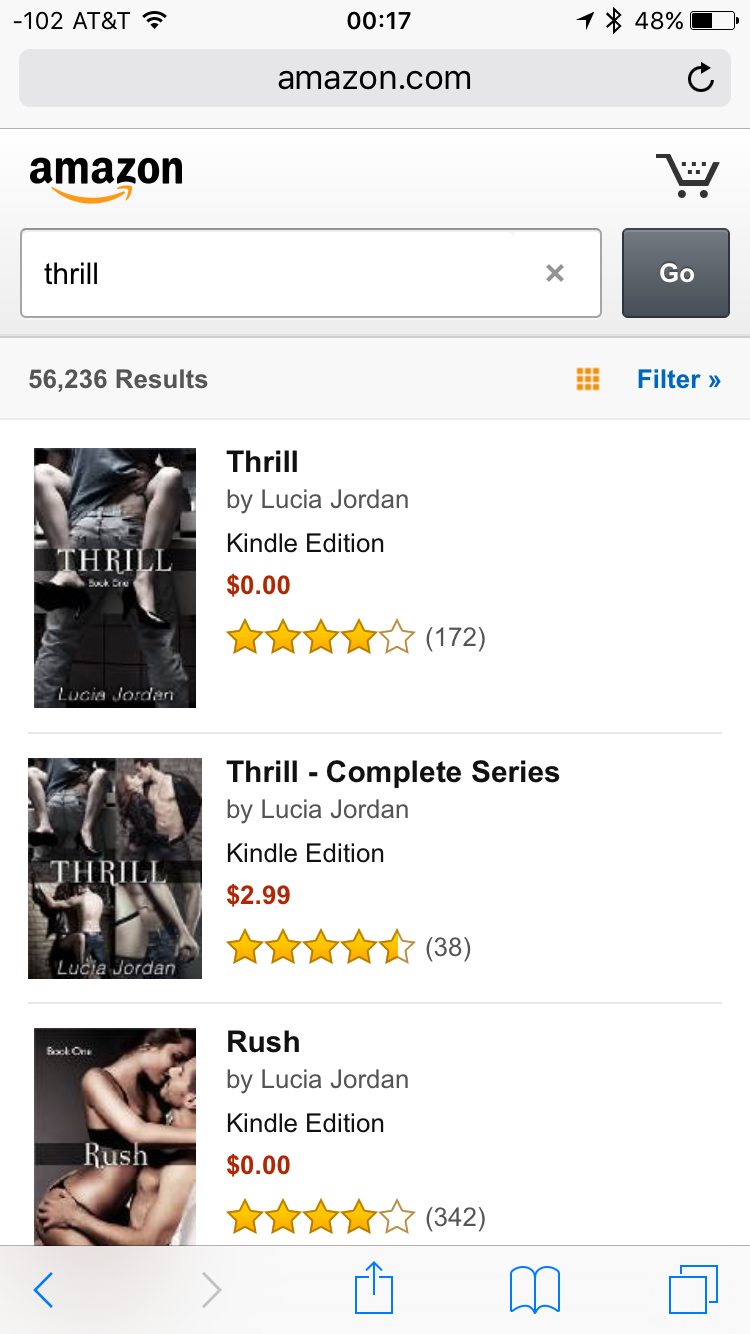
\includegraphics[width=8cm]{kindleDownload}
		% Create a subtitle for the figure.
		\caption{The results for a search of "Thrill" using the mobile \emph{amazon.com} site to search for Kindle books.}
		% Define the label of the figure. It's good to use 'fig:title', so you know that the label belongs to a figure.
		\label{fig:kindleDownload}
		\end{center}
	\end{figure}
    
    \begin{table}[!hbt]
		% Center the table
		\begin{center}
		% Title of the table
		\caption{"Download a book" (Kindle)}
		\label{tab:task1learnKindle}
		% Table itself: here we have two columns which are centered and have lines to the left, right and in the middle: |c|c|
		\begin{tabular}{|c|c|c|c|}
			% To create a horizontal line, type \hline
			\hline
			% To end a column type &
			% For a linebreak type \\
			$User$ & $Time$ $(sec)$ & $Errors$ & $Comments$\\
			\hline
            Albert & 20 & 0 & "Exciting"\\
			\hline
			Alex & 21 & 0 & "Annoying to go to browser"\\
			\hline
            Andrew & 18 & 0 & "Annoyed to use browser"\\
			\hline
			Eko & 19 & 0 & "No live results"\\
			\hline
            Harris & 125 & 1 & "Dumb, frustrating"\\
			\hline
			Josh & 13 & 0 & "I used Google"\\
			\hline
            Julia & 18 & 0 & "Same basic process"\\
			\hline
            Justin & 26 & 0 & "Would be nice to use app"\\
			\hline
            Lauren & 19 & 0 & "The cover made me want to read"\\
			\hline
            Maurice & 34 & 0 & "Inferior to iBooks"\\
			\hline
            Ronald & 24 & 0 & "Really stupid"\\
			\hline
            Sam & 15 & 0 & "Inconvenient, no in-app purchases"\\
			\hline
            Tori & 14 & 0 & "No American has time for that"\\
			\hline
		\end{tabular}
		\end{center}
	\end{table}
   
\subsection{Task 2: Highlight \& Note}
    The next task focused on a special feature available on both applications: highlighting and note-taking. Users were asked to simply highlight a section of text then add a note to the selected text. The basic touch gesture was similar on both applications, but the options that the gesture brings up are slightly different, as one can see from figures~\ref{fig:ibooksHighlight} and~\ref{fig:kindleHighlight}. These variations led to interesting results as some users were confused or hesitant while attempting to complete the task. Tables~\ref{tab:task2learniBooks} and~\ref{tab:task2learnKindle} illustrate the results for this task.
    
    \begin{table}[!hbt]
		% Center the table
		\begin{center}
		% Title of the table
		\caption{"Highlight \& Note" (iBooks)}
		\label{tab:task2learniBooks}
		% Table itself: here we have two columns which are centered and have lines to the left, right and in the middle: |c|c|
		\begin{tabular}{|c|c|c|c|}
			% To create a horizontal line, type \hline
			\hline
			% To end a column type &
			% For a linebreak type \\
			$User$ & $Time$ $(sec)$ & $Errors$ & $Comments$\\
			\hline
            Albert & 122 & 1 & "Unfortunate and unnatural"\\
			\hline
			Alex & 6 & 0 & "Similar to Google Books"\\
			\hline
            Andrew & 15 & 0 & "Likes magnifying glass"\\
			\hline
			Eko & 10 & 0 & "I feel fulfilled"\\
			\hline
            Harris & 15 & 0 & "Intuitive"\\
			\hline
			Josh & 20 & 0 & "It took a couple seconds"\\
			\hline
            Julia & 38 & 1 & "Really frustrating"\\
			\hline
            Justin & 39 & 1 & "Not intuitive"\\
			\hline
            Lauren & 9 & 1 & "Not as easy as expected"\\
			\hline
            Maurice & 21 & 0 & "Pleasant enough"\\
			\hline
            Ronald & 15 & 0 & "Pretty apparent how to do it"\\
			\hline
            Sam & 41 & 1 & "Text selection misleading"\\
			\hline
            Tori & 16 & 0 & "Very neat little quality"\\
			\hline
		\end{tabular}
		\end{center}
	\end{table}
    
    \begin{table}[!hbt]
		% Center the table
		\begin{center}
		% Title of the table
		\caption{"Highlight \& Note" (Kindle)}
		\label{tab:task2learnKindle}
		% Table itself: here we have two columns which are centered and have lines to the left, right and in the middle: |c|c|
		\begin{tabular}{|c|c|c|c|}
			% To create a horizontal line, type \hline
			\hline
			% To end a column type &
			% For a linebreak type \\
			$User$ & $Time$ $(sec)$ & $Errors$ & $Comments$\\
			\hline
            Albert & 17 & 1 & "Instinctual"\\
			\hline
			Alex & 13 & 0 & "Didn't work"\\
			\hline
            Andrew & 27 & 1 & "Quick to pick up"\\
			\hline
			Eko & 13 & 0 & "This is dumb"\\
			\hline
            Harris & 15 & 1 & "Not as intuitive as iBooks"\\
			\hline
			Josh & 19 & 0 & "Liked the color choices"\\
			\hline
            Julia & 18 & 0 & "Much easier"\\
			\hline
            Justin & 19 & 1 & "No default highlighting"\\
			\hline
            Lauren & 6 & 0 & "Two icons looked similar"\\
			\hline
            Maurice & 19 & 0 & "iBooks is more natural"\\
			\hline
            Ronald & 20 & 1 & "Pretty similar to iOS"\\
			\hline
            Sam & 14 & 0 & "In-text highlight more obvious"\\
			\hline
            Tori & 13 & 0 & "Different but similar options"\\
			\hline
		\end{tabular}
		\end{center}
	\end{table}
    
\subsection{Task 3: Find a Quote}
	The final task highlighted one of the most significant differences in design between the two applications. Users were asked to search for the quote: "Brandon Maxwell was no ordinary man." As one can infer from figures~\ref{fig:ibooksSearch},~\ref{fig:kindleSearch1}, and~\ref{fig:kindleSearch2}, the search function can be accessed in different locations depending on the application being used. The comments that arose from this task in particular were telling as to which application was preferred for this task. Results can be seen in tables~\ref{tab:task3learniBooks} and~\ref{tab:task3learnKindle}.
    
    \begin{table}[!hbt]
		% Center the table
		\begin{center}
		% Title of the table
		\caption{"Find a Quote" (iBooks)}
		\label{tab:task3learniBooks}
		% Table itself: here we have two columns which are centered and have lines to the left, right and in the middle: |c|c|
		\begin{tabular}{|c|c|c|c|}
			% To create a horizontal line, type \hline
			\hline
			% To end a column type &
			% For a linebreak type \\
			$User$ & $Time$ $(sec)$ & $Errors$ & $Comments$\\
			\hline
            Albert & 24 & 0 & "It was ordinary"\\
			\hline
			Alex & 12 & 0 & "Keyboard was difficult"\\
			\hline
            Andrew & 16 & 0 & "About what I expected"\\
			\hline
			Eko & 11 & 0 & "Enjoyed search bar"\\
			\hline
            Harris & 12 & 0 & "Standard search"\\
			\hline
			Josh & 11 & 0 & "Easy"\\
			\hline
            Julia & 8 & 0 & "Extremely easy"\\
			\hline
            Justin & 13 & 0 & "Literally a search button"\\
			\hline
            Lauren & 17 & 0 & "I made a typo"\\
			\hline
            Maurice & 15 & 0 & "Surprised"\\
			\hline
            Ronald & 12 & 0 & "Really easy"\\
			\hline
            Sam & 17 & 0 & "Easy and intuitive"\\
			\hline
            Tori & 10 & 0 & "It found it for me"\\
			\hline
		\end{tabular}
		\end{center}
	\end{table}
    
    \begin{figure}[!hbt]
		% Center the figure.
		\begin{center}
		% Include the eps file, scale it such that it's width equals the column width. You can also put width=8cm for example...
		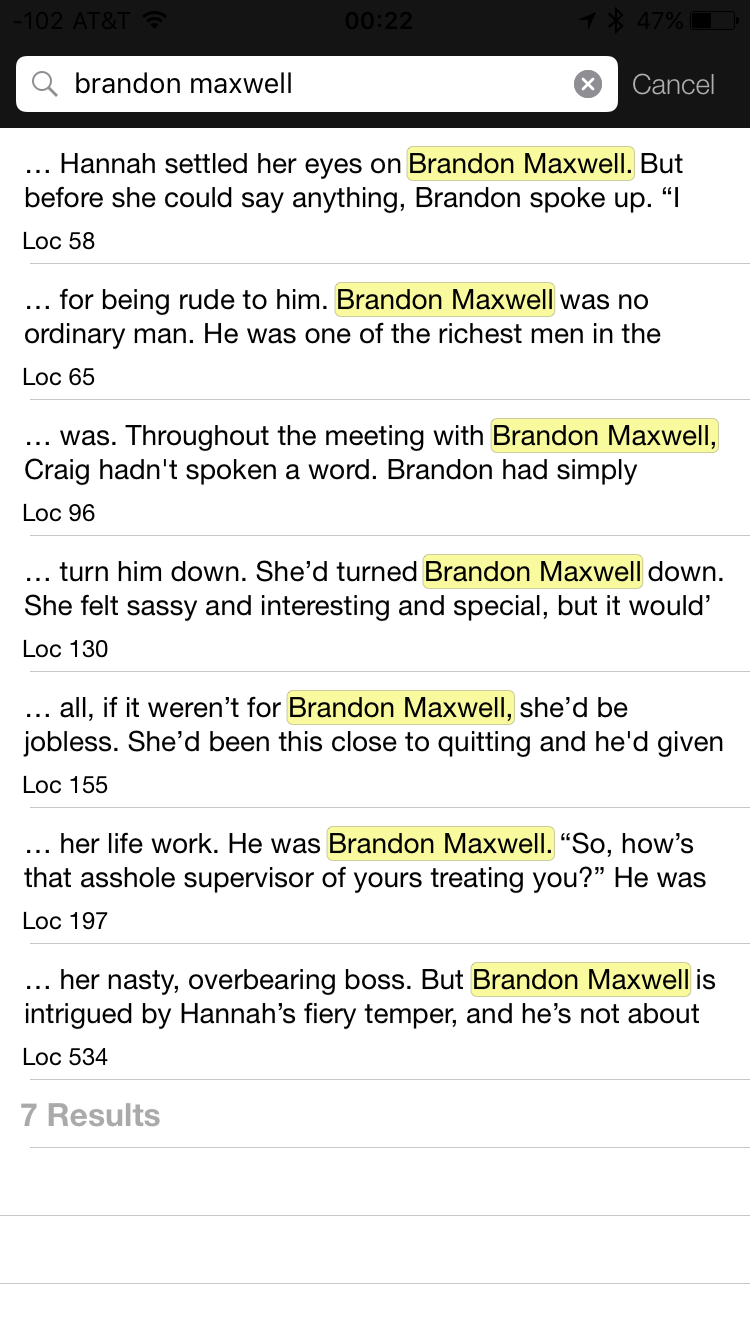
\includegraphics[width=8cm]{kindleSearch2}
		% Create a subtitle for the figure.
		\caption{After typing in the desired query, users needed to touch the "search" button to initiate the search in the Kindle application.}
		% Define the label of the figure. It's good to use 'fig:title', so you know that the label belongs to a figure.
		\label{fig:kindleSearch2}
		\end{center}
	\end{figure}
    
    \begin{table}[!hbt]
		% Center the table
		\begin{center}
		% Title of the table
		\caption{"Find a Quote" (Kindle)}
		\label{tab:task3learnKindle}
		% Table itself: here we have two columns which are centered and have lines to the left, right and in the middle: |c|c|
		\begin{tabular}{|c|c|c|c|}
			% To create a horizontal line, type \hline
			\hline
			% To end a column type &
			% For a linebreak type \\
			$User$ & $Time$ $(sec)$ & $Errors$ & $Comments$\\
			\hline
            Albert & 28 & 1 & "Bewitching"\\
			\hline
			Alex & 13 & 0 & "Keyboard issues"\\
			\hline
            Andrew & 33 & 1 & "Annoyed with menu button"\\
			\hline
			Eko & 8 & 0 & "Too many steps"\\
			\hline
            Harris & 21 & 1 & "Search was hidden"\\
			\hline
			Josh & 15 & 1 & "Kind of weird"\\
			\hline
            Julia & 17 & 1 & "Menus more hidden"\\
			\hline
            Justin & 17 & 0 & "Same as iBooks"\\
			\hline
            Lauren & 15 & 1 & "Lost at the start"\\
			\hline
            Maurice & 39 & 1 & "Easy"\\
			\hline
            Ronald & 21 & 1 & "Not instinctual"\\
			\hline
            Sam & 35 & 1 & "Didn't know where to search"\\
			\hline
            Tori & 80 & 1 & "Didn't live search"\\
			\hline
		\end{tabular}
		\end{center}
	\end{table}
    
	% If you have questions about how to write mathematical formulas in LaTeX, please read a LaTeX book or the 'Not So Short Introduction to LaTeX': tobi.oetiker.ch/lshort/lshort.pdf

\section{Heuristic Evaluation}
\subsection{Corresponding Guidelines Documentation}
	First we can use the existing documentation regarding specific guidelines from each developer to see how well the applications complied with their respective guidelines.
\subsubsection{iOS Human Interface Guidelines}
	According to Apple, Inc., iOS embodies the following themes: Deference, Clarity and Depth. Deference is used in the sense that the UI helps people understand and interact with the content, but never competes with it. Clarity deals with legible text, precise icons, appropriate adornments, and a focus on functionality. Finally, depth is the use of visual layers and realistic motion to impart vitality and heighten people's delight and understanding. 
    One of the guidelines provided is to "use plenty of negative space," because it important content and functionality more noticeable and easier to understand. This guideline is practiced within the iBooks application, as seen in figure~\ref{fig:ibooksDownload}. This figure also demonstrates the practice of the guideline to "let color simplify the UI." The idea of this guideline is to use a key color|blue in this case|to highlight important state information and subtly indicate interactivity.
    
    \begin{figure}[!hbt]
		% Center the figure.
		\begin{center}
		% Include the eps file, scale it such that it's width equals the column width. You can also put width=8cm for example...
		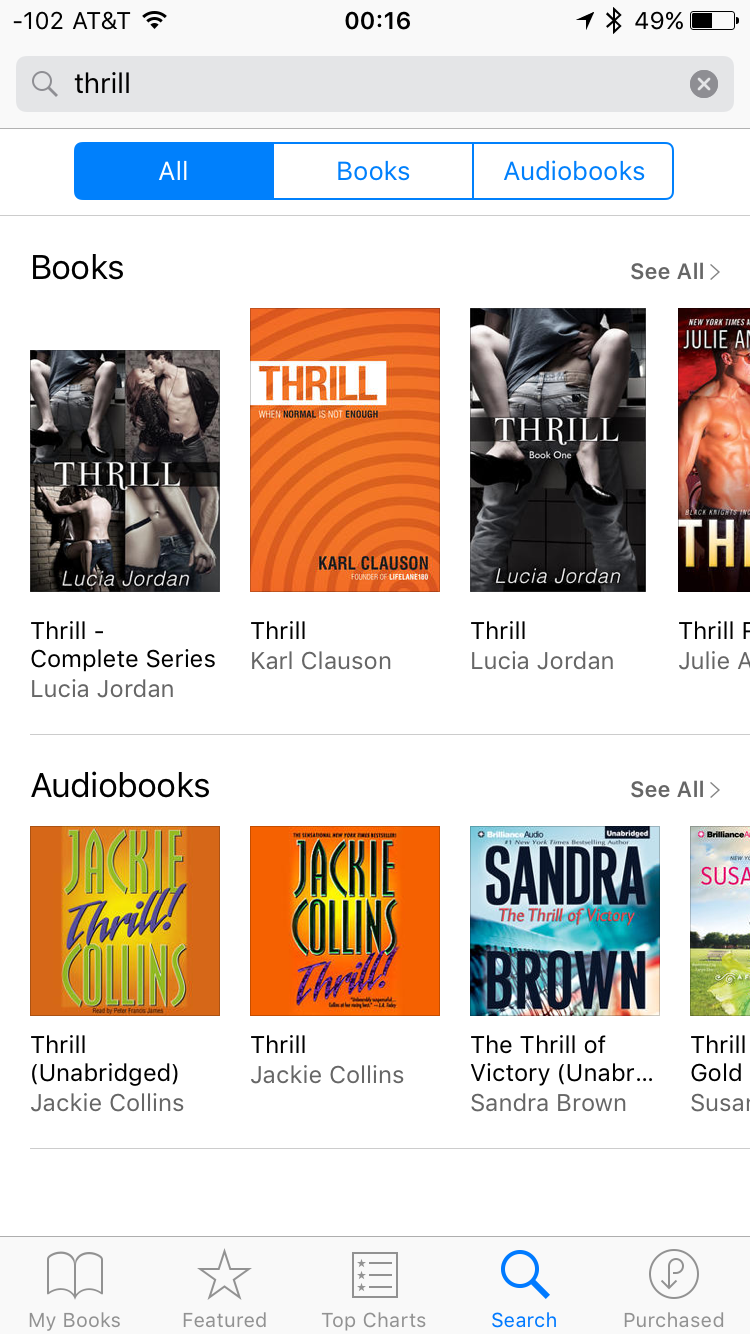
\includegraphics[width=8cm]{ibooksDownload}
		% Create a subtitle for the figure.
		\caption{The results for a search of "Thrill" in the in-app book search feature for iBooks.}
		% Define the label of the figure. It's good to use 'fig:title', so you know that the label belongs to a figure.
		\label{fig:ibooksDownload}
		\end{center}
	\end{figure}
    
    Another guideline or standard has to do with the fact that "users know the standard gestures." People generally expect gestures to work the same in all the apps they use. This expectation is assumed in the case of iBooks, as seen with our second task results, where many users simply touched and dragged across text to select it, a gesture that is consistent across iOS applications. A corollary guideline says to avoid defining new gestures unless the app is a game, which iBooks took to heart by keeping the default text-selection gesture. Figure~\ref{fig:ibooksHighlight} illustrates the outcome of this gesture.
    
    \begin{figure}[!hbt]
		% Center the figure.
		\begin{center}
		% Include the eps file, scale it such that it's width equals the column width. You can also put width=8cm for example...
		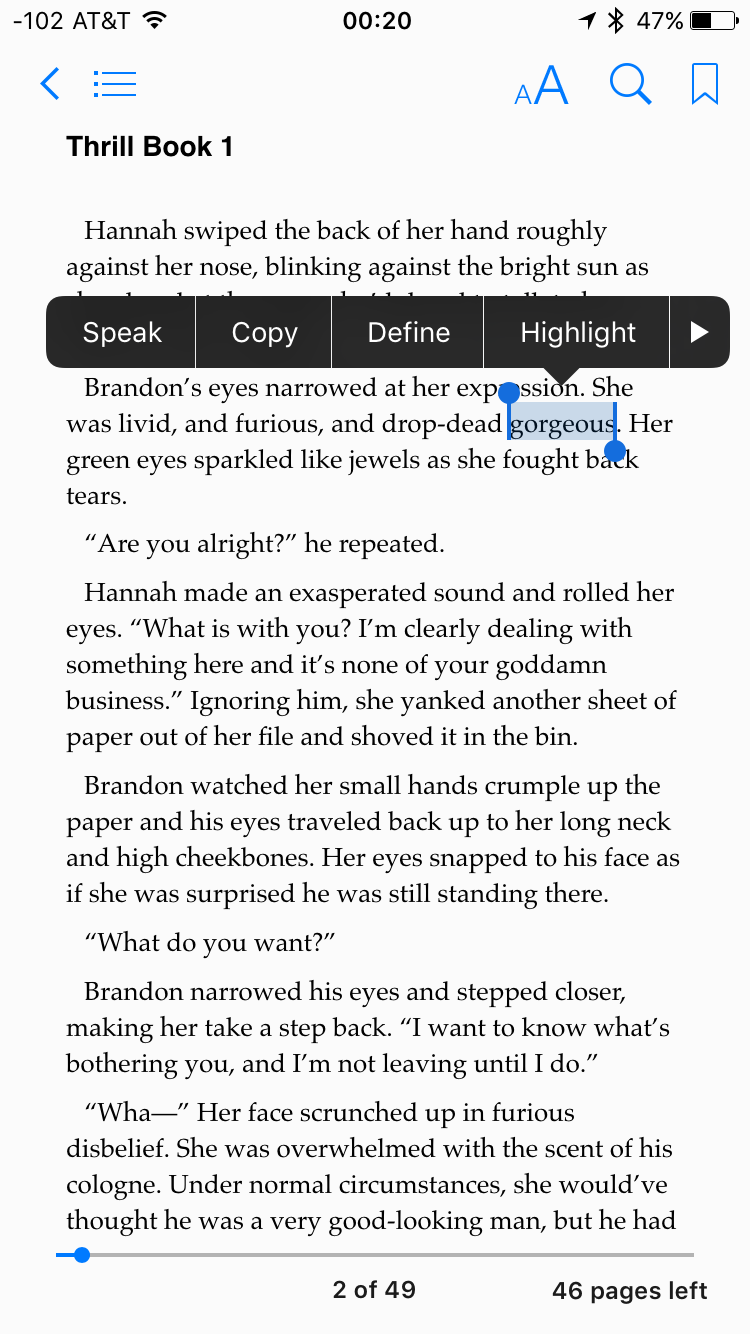
\includegraphics[width=8cm]{ibooksHighlight}
		% Create a subtitle for the figure.
		\caption{This is the small menu that appears after using a touch-and-hold gesture in iBooks.}
		% Define the label of the figure. It's good to use 'fig:title', so you know that the label belongs to a figure.
		\label{fig:ibooksHighlight}
		\end{center}
	\end{figure}
    
\subsubsection{Amazon Mobile Design Principles}
	Amazon has a specific set of principles for designing apps for their Fire Phone, from which the following guidelines were found. Amazon believes that the world is not flat, nor is it static, meaning that the real-world has depth and is in constant motion. In addition, they believe that the content shines brightest and simplicity should be a priority. Finally, their produces should exude the finest craftsmanship. These beliefs influence the way they make interaction design decisions.
    Under the touch gestures portion of the guidelines, the press and hold gesture is defined to begin drag and drop and/or show context menu. The Kindle application stays true to this defined guideline as the text-selection menu indeed appears after the user presses and holds the desired text. This implementation is shown in figure~\ref{fig:kindleHighlight}.
    
    \begin{figure}[!hbt]
		% Center the figure.
		\begin{center}
		% Include the eps file, scale it such that it's width equals the column width. You can also put width=8cm for example...
		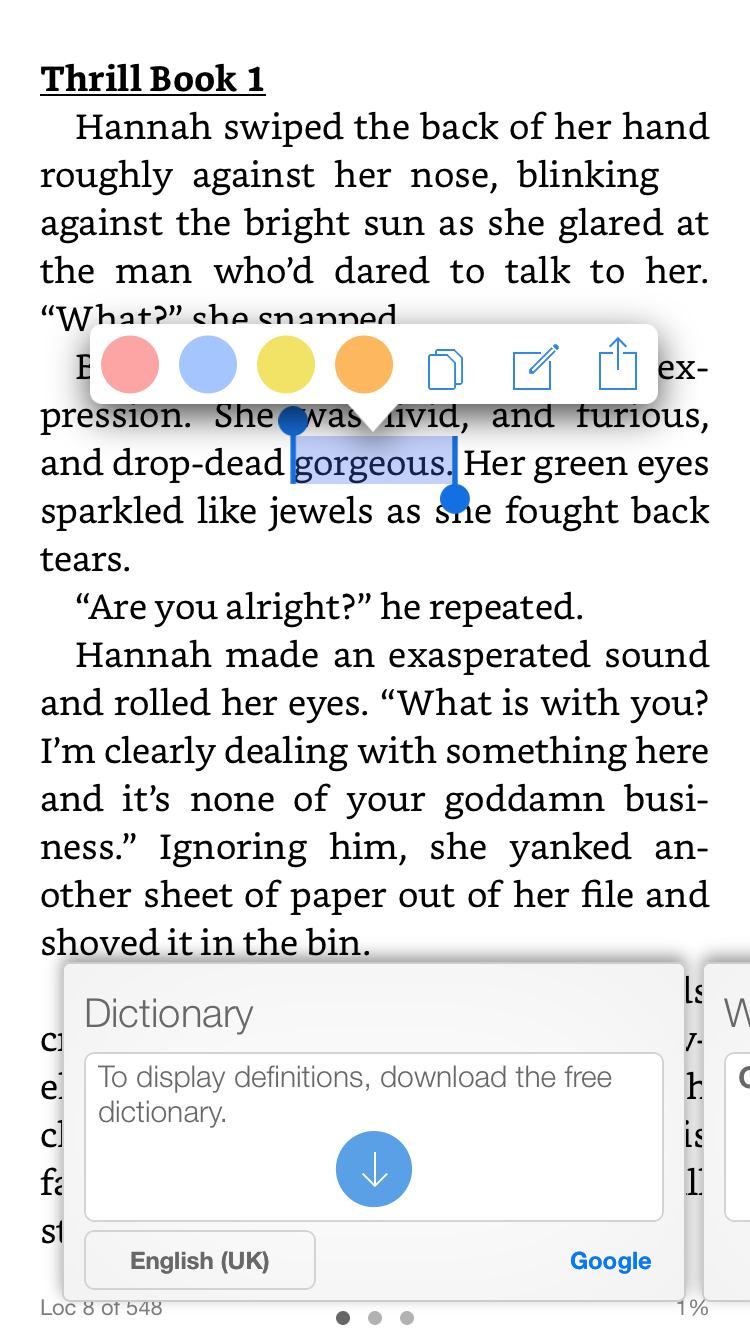
\includegraphics[width=8cm]{kindleHighlight}
		% Create a subtitle for the figure.
		\caption{This is the small menu that appears after using a touch-and-hold gesture in Kindle.}
		% Define the label of the figure. It's good to use 'fig:title', so you know that the label belongs to a figure.
		\label{fig:kindleHighlight}
		\end{center}
	\end{figure}
    
\subsection{Effectiveness of Pre-Dominant Interaction Styles}
	Looking deeper into the particular interaction design choices made by each developer, we can analyze and compare the choices to explain why iBooks performed better than Kindle.
\subsubsection{iBooks Interaction Design}
	The commentary we received from users indicated that the tasks were generally more intuitive and easier when done on iBooks, and after analyzing the results, it seems clear why this was the case. Many users were familiar with iOS interactions, and iBooks used these familiar and instinctive design concepts. For example, many mobile applications made by Apple have a live search feature accessible directly from the main screen, e.g. iTunes, App Store, etc. This same feature is available for both book searching and quote searching, which allows the user to press less buttons and type less words to find the desired object. In figure~\ref{fig:ibooksSearch}, the results shown were available in less than a second after the user typed "brandon maxwell." This sole feature differed greatly from the search feature available in Kindle, which did not have live search and was not immediately available to the user from the reading screen (Figure~\ref{fig:kindleSearch2}).
    Another obvious difference between the design of the two apps can be seen in the text selection menu. Apple has a guideline that specifically states that buttons or options must have text, with icons optional. This guideline can be seen throughout both iOS and Mac OS X, and manifests itself in figure~\ref{fig:ibooksHighlight}. In comparison, the Kindle text selection menu contains only icons and colored circles, which caused some issues at the user level because of the ambiguity of the copy icon, represented as two pieces of paper adjacent to one another (Figure~\ref{fig:kindleHighlight}).
    
    \begin{figure}[!hbt]
		% Center the figure.
		\begin{center}
		% Include the eps file, scale it such that it's width equals the column width. You can also put width=8cm for example...
		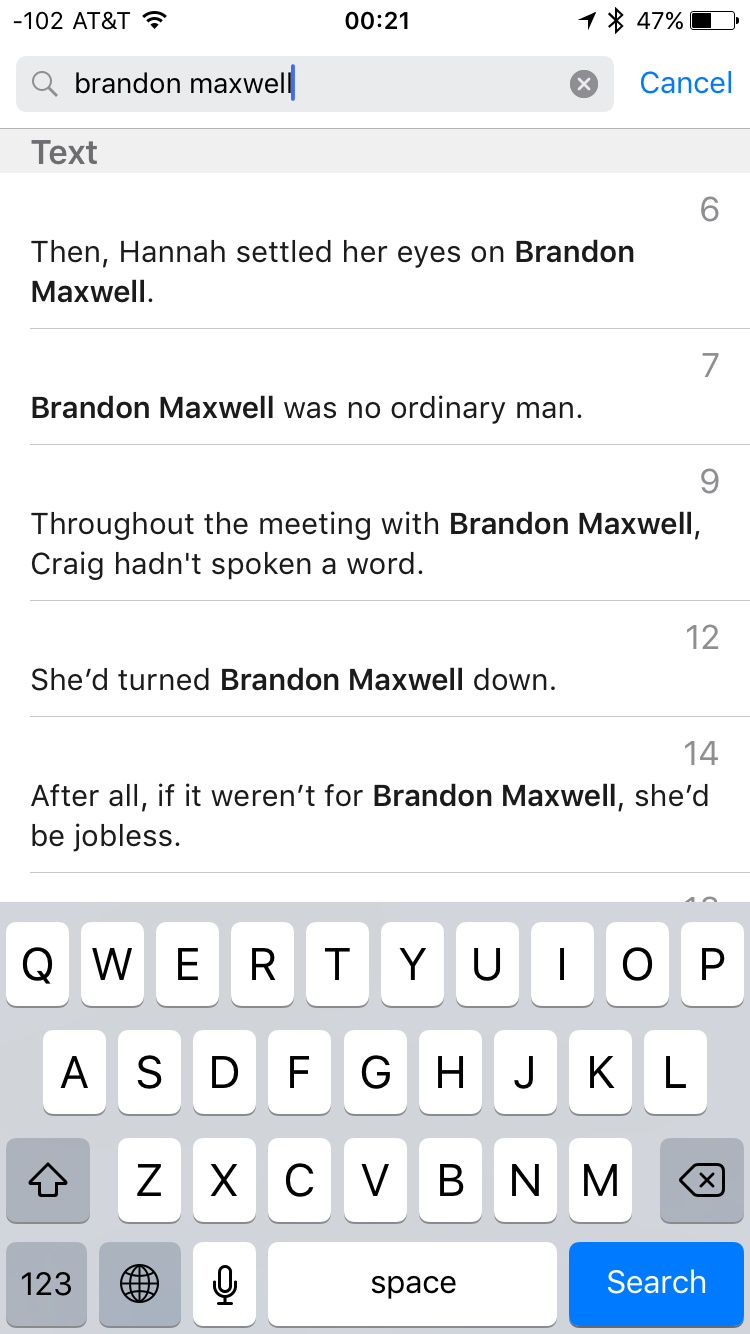
\includegraphics[width=8cm]{ibooksSearch}
		% Create a subtitle for the figure.
		\caption{After tapping the magnifying glass icon in the upper right-hand corner, this live search feature is activated in iBooks.}
		% Define the label of the figure. It's good to use 'fig:title', so you know that the label belongs to a figure.
		\label{fig:ibooksSearch}
		\end{center}
	\end{figure}
    
\subsubsection{Kindle Interaction Design}
	Although the Kindle application was found to be less user-friendly as a result of this report, the overall interaction design of the app was not completely inadequate. Although the text selection menu was confusing to some, users did like that the colored circles made it clear that the highlighted text would be that color. Giving explicit choice to the user is noteworthy, and a few users appreciated this. In addition, the Kindle application provided an optional dictionary feature that could be downloaded. Figure~\ref{fig:kindleHighlight} illustrates these features.
    One of the disadvantages Kindle faced was the home-field advantage possessed by iBooks, since the testing all occurred on an Apple device, namely an iPhone 6. Perhaps one of the most significant setbacks came to light in the first task, where users were forced to leave the app to find the book with Safari and Amazon.com. This is a monumental hindrance for both developers and users, because it takes the user out of the environment that can be controlled by the developer. In this case, one can only hope that the user has a pleasant experience with the mobile browser and that he/she will be willing to continue to use the app afterwards.
    One of the prominent differences between the mental models of both applications had to do with the menu placement and design. As with most other iOS apps, the menu for iBooks is placed on the bottom bar with five icons and descriptive text. This means near-instant access to any of the five options available to the user. However, the Kindle app uses another popular menu design concept where a second panel slides in from the left to reveal a list of options, with a couple having accompanying icons. When measuring both speed and satisfaction, we found that this implementation of a menu was slightly inferior because the search function was placed in this menu and not on the main screen. Some users spent a couple of seconds looking for the search button before finally opening the menu to find a rather hidden search button in the side menu, which is usually reserved for options pertaining to objects other than the one on the main screen. Figure~\ref{fig:kindleSearch1} shows how the Kindle menu looks after pressing the menu icon in the upper left hand corner.
    
    \begin{figure}[!hbt]
		% Center the figure.
		\begin{center}
		% Include the eps file, scale it such that it's width equals the column width. You can also put width=8cm for example...
		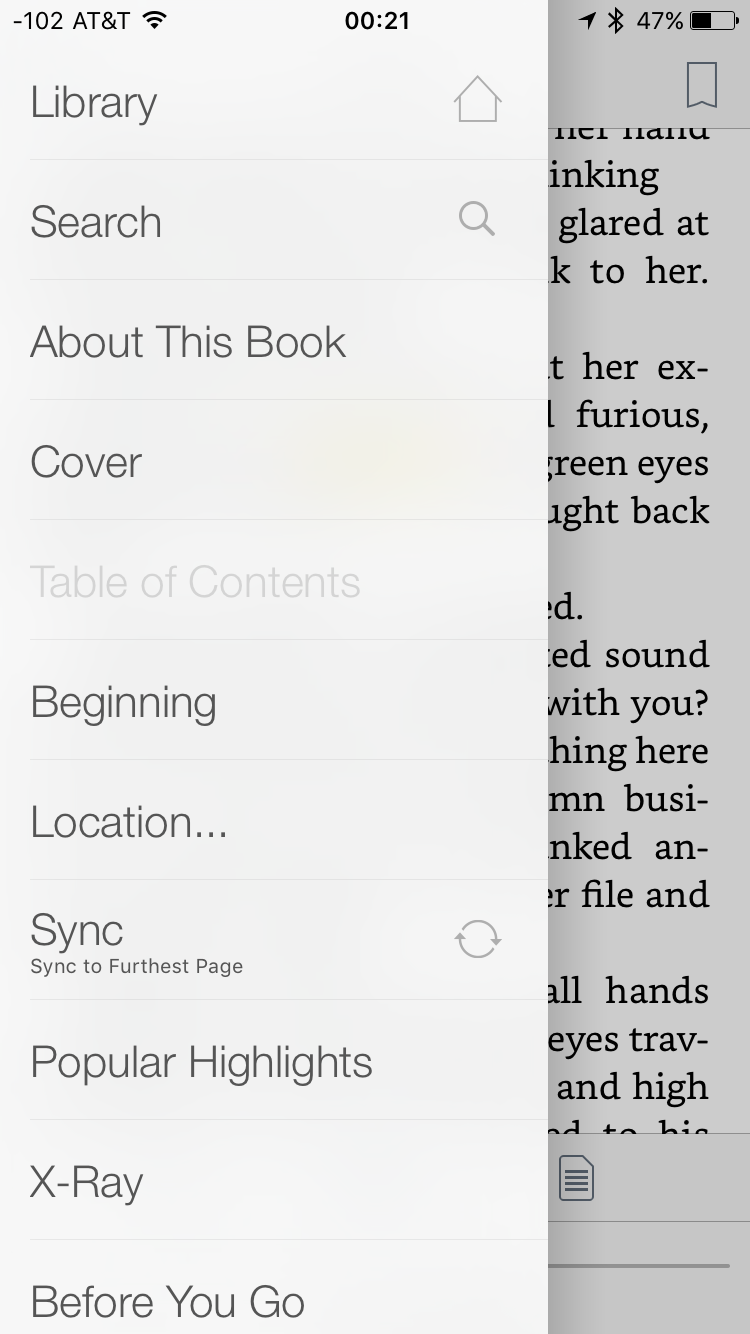
\includegraphics[width=8cm]{kindleSearch1}
		% Create a subtitle for the figure.
		\caption{Users needed to go into the side menu to find the search feature in the Kindle application.}
		% Define the label of the figure. It's good to use 'fig:title', so you know that the label belongs to a figure.
		\label{fig:kindleSearch1}
		\end{center}
	\end{figure}

\section{Conclusion}
	Learnability, errors, and satisfaction were measured in this report and the weighing of these metrics between the two applications resulted in iBooks being the preferred reading app. However, this study did not measure efficiency or memorability, two usability metrics that are arguably just as important, if not more important, than the three used for this report. With this being said, it is not difficult to see why iBooks performed better with test subjects. Learnability was not an issue for most users, since the feel of iOS is ubiquitous among younger users. Consistency was the name of the game for iBooks, as many tasks were deemed too simple because of the use of iOS-standard gestures and design. Errors were few and far between, and were often made due to typos or general confusion. Lastly, overall satisfaction with iBooks was high, with many citing the instinctive features as well as the easy navigation as reasons why they liked their experience.

% Now we need a bibliography:
\begin{thebibliography}{5}

	%Each item starts with a \bibitem{reference} command and the details thereafter.
	\bibitem{iOS}
	"iOS Human Interface Guidelines: Designing for iOS." iOS Developer Library. Apple, Inc., n.d. Web. 24 Sept. 2015.

	\bibitem{Amazon}
	"Design Principles - Amazon Apps \& Services Developer Portal." Amazon Developer Tools. Amazon.com, Inc., n.d. Web. 24 Sept. 2015.


\end{thebibliography}

% Your document ends here!
\end{document}